%% The first command in your LaTeX source must be the \documentclass command.
\documentclass[sigplan,screen]{acmart}
\usepackage{tikz}
\usetikzlibrary{positioning, arrows.meta, fit, backgrounds, calc}

%% \BibTeX command to typeset BibTeX logo in the docs
\AtBeginDocument{%
  \providecommand\BibTeX{{%
    Bib\TeX}}}

%% Rights management information.
\setcopyright{none}
\copyrightyear{2026}
\acmYear{2026}
\acmDOI{}

%% These commands are for a PROCEEDINGS abstract or paper.
\acmConference[CS 450]{}{March 28, 2026}{}
\acmISBN{}


%%
%% end of the preamble, start of the body of the document source.
\begin{document}

%%
%% The "title" command has an optional parameter,
%% allowing the author to define a "short title" to be used in page headers.
\title{Low-Latency Megakernels for LLM Inference}

%%
%% The "author" command and its associated commands are used to define
%% the authors and their affiliations.
\author{Andy Cheng}
\authornote{21232618}
\affiliation{%
  \institution{University of Waterloo}
  \country{Canada}
}

\author{Mischa Lamoureux}
\authornote{20938543}
\affiliation{%
  \institution{University of Waterloo}
  \country{Canada}
}

\author{Jatin Mehta}
\authornote{20940224}
\affiliation{%
  \institution{University of Waterloo}
  \country{Canada}
}

\author{Bilal Nasar}
\authornote{20944062}
\affiliation{%
  \institution{University of Waterloo}
  \country{Canada}
}

\author{Rishabh Sharma}
\authornote{20941002}
\affiliation{%
  \institution{University of Waterloo}
  \country{Canada}
}

\author{Andre Slavescu}
\authornote{20942887}
\affiliation{%
  \institution{University of Waterloo}
  \country{Canada}
}

%%
%% By default, the full list of authors will be used in the page
%% headers. Often, this list is too long, and will overlap
%% other information printed in the page headers. This command allows
%% the author to define a more concise list
%% of authors' names for this purpose.
\renewcommand{\shortauthors}{Cheng et al.}

\begin{abstract}
  Running large language models (LLMs) in single-sequence settings can be difficult because modern inference engines break the forward pass of a transformer into hundreds of small GPU kernels. Each kernel introduces overhead, which includes launch latency, synchronization, and unnecessary round-trips to global memory, all of which stall the GPU and waste memory bandwidth. Hazy Research recently showed that fusing an entire Llama-1B forward pass into a single \textit{megakernel} eliminates these pipeline bubbles and outperforms popular serving engines like vLLM and SGLang by over 1.5x on an Nvidia H100 GPU. We build on this idea in two ways: extending it to the Qwen3 model family to explore the generalizability of the megakernel approach, and optimizing specifically for Nvidia's newer Blackwell B200 GPU.

  For the Qwen3-1.7B model~\cite{qwen3}, we fuse all 28 decoder layers into a single kernel launch, handling Qwen3-specific features like per-head query/key normalization, grouped-query attention (GQA), and tied word embeddings. On a B200~\cite{blackwell}, this achieves 2.0-4.9 ms time-to-first-token (TTFT) across prompt lengths of 16-1024 tokens, which is a 6x improvement over vLLM~\cite{vllm} and SGLang~\cite{sglang}. We also scale the approach to Qwen3-480B-A35B, a 160-expert Mixture-of-Experts (MoE) model~\cite{shazeer2017moe}, with a fused 3-stage pipeline across 8 B200s using Blackwell-native tensor core and memory instructions. Our results show that the megakernel paradigm generalizes well beyond Llama-style architectures, and that designing kernels specifically for Blackwell, rather than porting from the older Hopper (H100) architecture, is key to squeezing out the most performance from modern hardware.
\end{abstract}


%%
%% This command processes the author and affiliation and title
%% information and builds the first part of the formatted document.
\maketitle


\section{Introduction}
\section{Background and Motivation}

Autoregressive decoding in decoder-only LLMs generates one token per forward pass, where each token depends on all preceding tokens. Each forward pass performs matrix multiplication (GEMVs) across all model layers (operations that are heavily memory-bandwidth bound rather than compute bound). The key performance metric is time-to-first-token (TTFT), which the user perceives as latency when interacting with these LLMs.


A decode step in a transformer executes hundreds of fine-grained CUDA kernels: normalization, QKV projections, attention, output projections, etc. which are repeated across every layer. Each kernel launch incurs setup and teardown overhead, and forces intermediate activations to be written to and read from memory between operations. On an H100, launch overhead alone can consume hundreds of microseconds, which is a significant fraction of the total decode latency for small models and the GPU spends more time waiting than computing.


Hazy Research introduced a megakernel architecture that fuses the entire transformer decode pass into a single persistent kernel launch~\cite{hazyresearch}. By keeping all intermediate activations in shared memory (vs ${\sim}$3.35\,TB/s for memory) and eliminating kernel boundaries, the megakernel removes the repeated global memory round-trips and launch overhead. Their implementation for Llama-1B on H100 demonstrated significant speedups over production serving engines like vLLM and SGLang. The kernel uses an instruction-driven execution model where a controller warp fetches and dispatches operations to specialized worker warps, with a shared memory page allocator managing on-chip tensor storage.


Despite its strong results, the Hazy Research megakernel has three key limitations. First, their B200 implementation underexploits the Blackwell architecture; the authors themselves report that approximately 250$\mu$s (40\% of total runtime) is spent on activation store/load overhead, noting their B200 results are ``quite a ways off from the theoretical limit.'' Blackwell introduces dedicated tensor memory with explicit alloc/dealloc lifecycle, 2-CTA cluster execution, and new generation tensor core instructions (tcgen05). Second, the implementation is specialized exclusively for the Llama-1B architecture and does not generalize to other model families or to sparse Mixture-of-Experts (MoE) architectures, which are increasingly dominant in production LLMs. Third, synchronization overhead from their counter-based global memory barriers and standard CUDA barriers leaves measurable performance on the table.


These limitations motivate our work to have a megakernel inference engine designed from the ground up for NVIDIA Blackwell B200 GPUs, extended to the Qwen3 model family spanning both dense (1.7B) and MoE (480B-A35B) architectures. By exploiting B200-specific features such as tcgen05 tensor core instructions, tensor memory, CTA cluster cooperation, and cluster-scoped TMA and by demonstrating generality across fundamentally different model architectures, we aim to push megakernel inference by leveraging newer generation hardware.

\section{High-Level Ideas}

Our approach rests on three pillars: (1) fusing the entire dense transformer into a single persistent kernel, (2) extending the megakernel paradigm to sparse Mixture-of-Experts architectures, and (3) exploiting Blackwell-specific hardware features throughout. Figure~\ref{fig:pipeline} illustrates the overall pipeline for the dense model.

\paragraph{Persistent dense megakernel.}
For Qwen3-1.7B, we fuse all 28 decoder layers into one cooperative kernel launch on 128 thread blocks, eliminating the 200+ kernel launches that PyTorch eager mode requires. Thread blocks are statically specialized: one coordinator block manages KV cache pointers, 16 blocks handle grouped-query attention (one per Q head), and 111 blocks perform the FFN GEMVs. All intermediate activations stay in shared memory, and layers are chained through lightweight global-memory grid barriers, so no intermediate results ever round-trip through HBM. We detail this architecture in Section~\ref{sec:dense}.

\paragraph{MoE scaling.}
To scale beyond dense models, we extend the megakernel idea to Qwen3-480B-A35B, a 160-expert MoE model distributed across 8 B200 GPUs. The MoE FFN is restructured as a 3-stage fused pipeline: (i) a single-kernel router that computes gating logits, selects top-8 experts, and sorts tokens by expert, (ii) a persistent tcgen05 gate-up GEMM with fused SiLU activation, and (iii) a persistent tcgen05 down GEMM with weighted scatter-accumulate. This replaces what would otherwise be 8+ separate kernel launches per MoE layer. Expert parallelism (EP=8) places 20 experts per GPU, while tensor parallelism (TP=8) shards the attention layers. The full MoE design is described in Section~\ref{sec:moe}.

\paragraph{Blackwell-native optimizations.}
Rather than porting Hopper (H100) kernels, we design for the B200 from the ground up. The expert GEMMs use \texttt{tcgen05} 5th-generation tensor core instructions with dedicated tensor memory and 2-CTA cluster execution, where each cluster CTA loads half the weight tile and multicasts to its partner via cluster-scoped TMA, halving weight-load bandwidth. Prefill attention uses a CUTLASS SM100 FMHA kernel exploiting the B200's larger register file and doubled shared memory. Additional optimizations---replacing the custom router with a cuBLAS GEMM (6$\times$ speedup), vectorizing elementwise kernels with \texttt{float4} loads, and moving the prefix scan to the GPU---collectively reduce per-layer MoE latency by 49\%. These optimizations are detailed in Sections~\ref{sec:b200} and~\ref{sec:addopt}.

\begin{figure}[h]
  \centering
  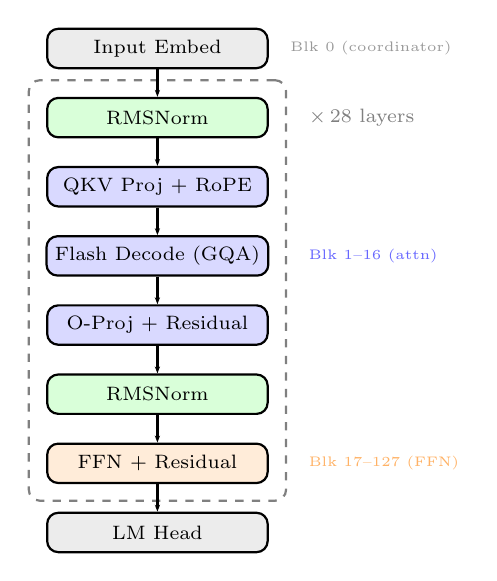
\begin{tikzpicture}[
    node distance=0.35cm,
    block/.style={draw, rounded corners, minimum height=0.5cm, minimum width=2.8cm, font=\scriptsize, inner sep=3pt, thick},
    attn/.style={block, fill=blue!15},
    ffn/.style={block, fill=orange!15},
    norm/.style={block, fill=green!15},
    io/.style={block, fill=gray!15},
    layerbox/.style={draw, dashed, rounded corners, inner sep=6pt, thick, gray},
    arr/.style={-{Stealth[length=2.5pt]}, thick},
    lbl/.style={font=\tiny, anchor=west},
  ]
    % Input
    \node[io] (input) {Input Embed};

    % Layer ops - vertical stack
    \node[norm, below=of input] (rms1) {RMSNorm};
    \node[attn, below=of rms1] (qkv) {QKV Proj + RoPE};
    \node[attn, below=of qkv] (attn) {Flash Decode (GQA)};
    \node[attn, below=of attn] (oproj) {O-Proj + Residual};
    \node[norm, below=of oproj] (rms2) {RMSNorm};
    \node[ffn, below=of rms2] (ffn) {FFN + Residual};

    % Arrows
    \draw[arr] (input) -- (rms1);
    \draw[arr] (rms1) -- (qkv);
    \draw[arr] (qkv) -- (attn);
    \draw[arr] (attn) -- (oproj);
    \draw[arr] (oproj) -- (rms2);
    \draw[arr] (rms2) -- (ffn);

    % Layer box
    \begin{scope}[on background layer]
      \node[layerbox, fit=(rms1)(qkv)(attn)(oproj)(rms2)(ffn)] (layer) {};
    \end{scope}

    % Block labels to the right of the layer box
    \node[lbl, gray!80, right=0.15cm of input] {Blk 0 (coordinator)};
    \node[lbl, blue!60, right=0.15cm of layer.east |- attn] {Blk 1--16 (attn)};
    \node[lbl, orange!60, right=0.15cm of layer.east |- ffn] {Blk 17--127 (FFN)};
    \node[font=\scriptsize, gray, right=0.15cm of layer.east |- rms1] {$\times\,28$ layers};

    % Output
    \node[io, below=of ffn] (lmhead) {LM Head};
    \draw[arr] (ffn) -- (lmhead);
  \end{tikzpicture}
  \caption{Dense megakernel pipeline for Qwen3-1.7B. All 28 layers execute within a single persistent kernel launch. Thread blocks are statically assigned to attention (blue) or FFN (orange) roles. All inter-layer data stays in shared memory.}
  \label{fig:pipeline}
\end{figure}

\section{Implementation and Mechanism}
\subsection{Dense Megakernel Architecture Qwen3 1.7B}
\label{sec:dense}

The core contribution for the dense model is a persistent megakernel that fuses all 28 transformer decoder layers into a single cooperative kernel launch. The kernel runs on a fixed grid of 128 blocks $\times$ 512 threads (65{,}536 threads total), launched via \texttt{cudaLaunchCooperativeKernel} to enable device-wide synchronization through a custom \newline \texttt{GridBarrier} built on global atomics.

\subsubsection{Block Specialization}

Rather than launching separate kernels per operation, the megakernel assigns functional roles to thread blocks at compile time. Block 0 acts as the KV cache coordinator, managing KV write pointers and synchronizing attention heads with FFN blocks via the grid barrier. Blocks 1 through 16 handle flash decode attention, with one block per query head (16 heads for 1.7B), where each block computes grouped-query attention (GQA ratio $= 2$, sharing 8 KV heads across 16 Q heads) using online softmax with warp-per-head decomposition. Within each block, warps chunk the KV sequence and maintain running \texttt{(max, sum, output)} accumulators that are merged via a final reduction in shared memory. The remaining blocks 17 through 127 serve as FFN GEMV workers, where 111 blocks collectively compute the gate/up/down projections via parallel row-wise dot products with vectorized 8-element \texttt{uint4} loads of BF16 pairs using \texttt{\_\_ldcg} (cache-global) for sustained bandwidth.

All inter-layer communication is barrier-mediated, with 5 grid barriers per layer (140 total for 28 layers) and intermediate activations residing in a single shared buffer of $(H + 32) \times 4 = 8{,}320$ bytes per block (where $H = 2{,}048$ for 1.7B). No intermediate results are written to global HBM between fused operations.

\subsubsection{Fused Operations}

\begin{table}[h]
  \caption{Fused operations eliminating HBM round-trips.}
  \label{tab:3}
  \small
  \begin{tabular}{lll}
    \toprule
    Fused Kernel & Operations & Saved \\
    \midrule
    rmsnorm\_qkv & RMSNorm + QKV proj + split & $4{\to}1$ \\
    qknorm\_rope & QK norm + RoPE + KV write & $5{\to}1$ \\
    flash\_decode & GQA attn (online softmax) & $3{\to}1$ \\
    oproj\_res & O-proj + residual add & $2{\to}1$ \\
    upgate\_silu & Gate/Up GEMV + SiLU + mul & $4{\to}1$ \\
    downproj\_res & Down proj + residual add & $2{\to}1$ \\
    rmsnorm\_lm & Final RMSNorm + LM head & $2{\to}1$ \\
    \bottomrule
  \end{tabular}
\end{table}

The total per forward pass is 1 megakernel launch plus 1 CUTLASS SM100 FMHA call (for prefill), giving 2 launches compared to over 200 with PyTorch eager mode. The FMHA kernel uses CUTLASS~\cite{cutlass} \texttt{Sm100FmhaFwdKernelTmaWarpspecialized} \newline with tile shape $\langle 256, 128, 128 \rangle$ (Q-seq $\times$ K-seq $\times$ head\_dim), TMA-based async global-to-shared loads, and a persistent tile scheduler.

\subsubsection{Qwen3-Specific Adaptations}

The kernel accounts for several Qwen3 architectural features not present in the Llama baseline. Per-head Q/K RMSNorm is applied after projection and before RoPE, fused into a single device function that avoids writing intermediate normalized values to HBM. For GQA with ratio 2, where 16 Q heads share 8 KV heads, the flash decode kernel maps $\lfloor \texttt{head\_idx} / 2 \rfloor$ to select the correct KV head, doubling compute reuse per KV cache read. The embedding matrix is also reused for the LM head via tied word embeddings, saving 300\,MB of weight memory for the 1.7B model.

\subsection{Scaling to Qwen3-480B-A35B: MoE Megakernel}
\label{sec:moe}

The Qwen3-Coder-480B-A35B model replaces the dense FFN with a Mixture-of-Experts (MoE) layer consisting of 160 routed experts with top-8 gating, a hidden size of 6{,}144, and a per-expert intermediate dimension of 2{,}560. At approximately 960 GB in BF16, the model requires 8$\times$ B200 GPUs with expert parallelism (EP=8), giving 20 local experts per GPU.

\subsubsection{3-Stage Kernel Pipeline}

The MoE FFN has been implemented as a 3-stage fused pipeline, replacing what would otherwise be 8+ separate kernel launches per MoE layer.

The first stage handles routing and sorting. A single kernel computes router logits via a warp-per-(token, expert) GEMV pattern ($[T, 6144] \times [160, 6144]^T$), applies numerically-stable softmax, selects the top-8 experts, and sorts tokens by local expert index via a histogram + scatter approach. This is optimal for the small expert count ($E=20$) and avoids the overhead of CUB radix sort.

The second stage performs the fused gate-up GEMM. A persistent tcgen05 kernel computes the gate-up projection, where each expert's gate and up weight matrices have been concatenated into a single $[5120, 6144]$ matrix, turning two GEMMs into one wider GEMM per expert. A fused SiLU activation kernel then computes $\text{SiLU}(\text{gate}) \odot \text{up}$ in a single pass.

The third stage handles the down GEMM and scatter. A second persistent tcgen05 kernel computes the down projection ($[2560 \rightarrow 6144]$), followed by a weighted scatter-accumulate that writes each expert's output back to the original token position with the routing weight applied, using FP32 atomic adds.

\subsubsection{Persistent tcgen05 Expert GEMM}

The expert \newline GEMM kernels are the computational core of the MoE layer. Built on the ThunderKittens~\cite{thunderkittens} B200 matmul framework, they use explicit \texttt{tcgen05} PTX inline assembly for all 5th-generation tensor core operations, including \newline \texttt{tcgen05.mma.cta\_group::2.kind::f16} \newline for BF16$\times$BF16$\rightarrow$FP32 matrix multiply-accumulate across a 2-CTA cluster, \texttt{tcgen05.commit} for signaling mbarrier completion with multicast to both cluster CTAs, \texttt{tcgen05.ld} with \texttt{pack::16b} for loading FP32 accumulators from tensor memory while packing to BF16, and \newline \texttt{tcgen05.fence::before/after\_thread\_sync} for memory ordering around barrier syncs.

\paragraph{Tile configuration.} Each task operates on $M_b = 128$ rows $\times$ $N_b = 256$ columns with $K_b = 64$ reduction per TMA load. A 2-CTA cluster processes $\text{CLUSTER\_M} = 512$ rows per task (4 consumer tiles, from 2 CTAs $\times$ 2 consumer warpgroups $\times$ 128 rows). The TMA pipeline depth is 4 stages, keeping the tensor cores fed while loads are in flight.

\paragraph{Warp specialization.} Each CTA runs 3 warpgroups (384 threads). Warpgroups 0 and 1 are the consumers, each with 224 registers, responsible for loading FP32 results from tensor memory via \texttt{tcgen05.ld}, converting to BF16, and storing to global memory via TMA. Warpgroup 2 is the producer with 56 registers, where warp 3 issues TMA \texttt{cp.async.bulk} loads for the A (activations) and B (weights) tiles, while warps 0 and 1 issue \texttt{tcgen05.mma} instructions. Phase-bit semaphores are used to synchronize the producer-consumer ring buffer.

\paragraph{Persistent task scheduler.} All (expert, $m$-tile, $n$-tile) combinations across the 20 local experts are flattened into a linear task queue. A global atomic counter distributes tasks to CTAs, achieving natural load balancing even when expert token counts are imbalanced. The scheduler uses binary search over prefix-summed expert tile offsets to decode each flat task ID into its (expert, $m$-tile, $n$-tile) triple. The kernel launches on 148 CTAs (74 clusters, matching the B200's 148 SMs) with maximum dynamic shared memory allocation.

\subsubsection{Expert Weight Packing}

To avoid scatter-gather overhead during the GEMM, expert weights are packed into contiguous buffers at model load time. The gate and up projection weights are concatenated per expert into a $[E_{\text{local}}, 2I, H] = [20, 5120, 6144]$ buffer, and the down projection weights are stored as $[E_{\text{local}}, H, I] = [20, 6144, 2560]$. The B matrix TMA descriptor flattens the expert dimension into the row dimension ($[E \cdot N, K]$), so the TMA load coordinate simply indexes \texttt{expert $\times$ stride + tile\_col}. After packing, the original \texttt{nn.Linear} modules are freed, preventing the approximately 109 GiB weight duplication that would otherwise cause OOM.

\subsubsection{Distributed Communication}

The 8-GPU setup uses two orthogonal parallelism strategies. For attention, tensor parallelism~\cite{megatronlm} (TP=8) is used, where Q/K/V heads are sharded across ranks with \texttt{all\_reduce} for the output projection, and each rank computes $96/8 = 12$ Q heads and $8/8 = 1$ KV head. For the MoE layer, expert parallelism (EP=8) is used, where each rank holds 20 of the 160 experts and partial outputs are combined via NCCL \texttt{all\_reduce} across the EP process group after local expert computation.

For the TP all-reduce, we additionally explored multimem NVLS (NVLink SHARP), which is a fused \texttt{ld\_reduce\_add\_bf16x8} kernel that performs all-reduce directly through NVLink multicast memory, bypassing NCCL's ring protocol. This provides lower latency for the small activation tensors typical of batch-1 decode (approximately $6{,}144 \times 2 = 12$ KB per all-reduce).

\subsection{B200 (SM100) Optimizations}
\label{sec:b200}

Several optimizations are specific to the Blackwell architecture. Unlike Hopper's \texttt{wgmma} which reads accumulators from registers, Blackwell's tcgen05 uses dedicated tensor memory with an explicit alloc/dealloc lifecycle. The \newline \texttt{tensor\_allocator<1,2>} manages column allocation across the 2-CTA cluster, and the \texttt{tcgen05.ld} instruction supports a \texttt{pack::16b} modifier that converts FP32 accumulator values to BF16 during the load, eliminating a separate conversion pass.

The B200's cluster architecture allows two CTAs to share data through cluster-scoped TMA loads \newline (\texttt{tma::cluster::load\_async} with a multicast mask). Each CTA loads its half of the B matrix (128 of 256 columns) and broadcasts to the partner CTA, halving the required TMA bandwidth for weights. The prefill attention path uses a CUTLASS SM100 FMHA kernel~\cite{flashattention} with persistent tile scheduling, achieving higher occupancy than the SM90 (Hopper) equivalent by exploiting the B200's larger register file (256 registers/thread) and doubled shared memory capacity (228 KB/SM). The scatter-accumulate kernel uses FP32 \texttt{atomicAdd} for weighted output accumulation, and on B200 these atomics execute at the L2 cache level with 2$\times$ the bandwidth of H100, reducing the scatter bottleneck for high fan-out routing (top-8 $\times$ $T$ tokens).

\subsection{Additional Kernel Optimizations}
\label{sec:addopt}

Beyond the persistent tcgen05 GEMM architecture, we applied three additional optimizations to the MoE pipeline that collectively reduced per-layer latency by 49\%.

\paragraph{cuBLAS router matmul.} The original router used a custom warp-per-(token, expert) kernel for the \newline $[T, 6144] \times [160, 6144]^T$ logit computation. Profiling revealed this consumed 44\% of non-GEMM time ($\sim$0.6\,ms at $T{=}4096$). Replacing it with a single cuBLAS GEMM call leverages B200 tensor cores and reduces this to $\sim$0.1\,ms, a 6$\times$ improvement for the router alone.

\paragraph{Vectorized elementwise kernels.} The gather, SiLU fusion, and scatter-accumulate kernels were rewritten with a row-per-block pattern using \texttt{float4} vectorized loads (8 BF16 values per thread per iteration). This improves memory throughput by $\sim$4$\times$ compared to the original scalar kernels.

\paragraph{GPU-side prefix scan.} The router pipeline originally performed a CPU-side exclusive prefix scan over the 20 expert token counts, requiring a device-to-host copy, CPU loop, host-to-device copy, and an explicit \texttt{cudaStreamSynchronize}. We replaced this with a single-block GPU kernel, eliminating one synchronization point per MoE layer.


\section{Evaluation}
In this section, we present the results of our reproduction of the Hazy megakernel, as well as our implementation of the megakernel architecture for the Qwen3-1.7B model and its scaling to the Qwen3-480B-A35B MoE model. We evaluate performance in terms of time-to-first-token (TTFT) across various prompt lengths, and compare against popular serving engines like vLLM and SGLang.
\subsection{Baseline Reproduction}
Reproduction of performance improvements of the Hazy Megakernel, as presented in their blogs have been successful. Reproduction was conducted using the H100s and B200s provided through the \textbf{Modal}~\cite{modal} cloud computing platform and invoking the benchmarking scripts as provided by the original authors, with minimal changes for code execution and environment compatibility, primarily in the form of \textbf{Docker} and \textbf{custom data collection scripts}. Figures describing our recovered results can be seen below in Figure~\ref{fig:1}, where similar results have been reproduced for both the H100 and B200, a discrepancy that was resolved from our prior checkpoint report. A final note is that Token/s in our figure are synonymous with Forward Passes (Fwd)/s with that of Hazy's.

\begin{figure}[h]
  \centering
  % Replace 'figure1.png' with your actual uploaded file name
  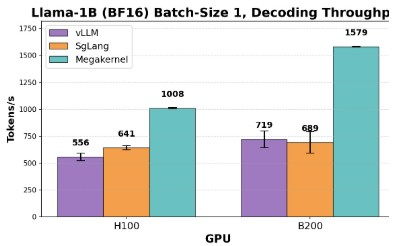
\includegraphics[width=\linewidth]{figure1.jpg}
  \caption{Reproduced baseline and mega-kernel results on both H100 and B200. Each bar graph is mean token/s over 3 iterations.}
  \label{fig:1}
\end{figure}

\begin{figure}[h]
  \centering
  % Replace 'figure2.png' with your actual uploaded file name
  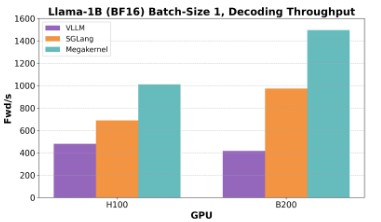
\includegraphics[width=\linewidth]{figure2.jpg}
  \caption{Baseline results from the blog}
  \label{fig:2}
\end{figure}

\subsection{Qwen3-1.7B}
Our persistent megakernel achieves 2.0-4.9ms TTFT across all prompt lengths on a single B200, compared to 14-19ms for production serving engines.

\begin{table}[h]
  \caption{Persistent megakernel vs baselines for Qwen3-1.7B on B200}
  \label{tab:1}
  \small
  \begin{tabular}{rrrr}
    \toprule
    Tokens & Ours (ms) & vLLM (ms) & SGLang (ms) \\
    \midrule
    16   & 2.02 & 14.28 & 16.15 \\
    64   & 2.23 & 13.91 & 14.70 \\
    128  & 2.36 & 16.45 & 15.59 \\
    256  & 2.64 & 14.15 & 14.87 \\
    512  & 3.28 & 15.45 & 15.22 \\
    1024 & 4.86 & 17.21 & 16.06 \\
    \bottomrule
  \end{tabular}
\end{table}

At 128 tokens input, we achieve 7.0x over vLLM and 6.6x over SGLang.

\begin{table}[h]
  \caption{Hardware utilization for our persistent megakernel on B200}
  \label{tab:2}
  \small
  \begin{tabular}{rrrr}
    \toprule
    Seq Len & Tok/s & BW (GB/s) & TF \\
    \midrule
    1    & 478 & 1645 (20.6\%) & 1.65 \\
    128  & 429 & 1484 (18.6\%) & 1.49 \\
    512  & 333 & 1165 (14.6\%) & 1.18 \\
    1024 & 256 & 912 (11.4\%)  & 0.94 \\
    \bottomrule
  \end{tabular}
\end{table}

The decode phase is memory-bandwidth bound (thin GEMVs), achieving up to 1645 GB/s of the B200's 8 TB/s peak.

\subsection{Qwen3-480B MoE Results}

\subsubsection{Single-GPU MoE Layer Performance}

Table~\ref{tab:moe-kernel} shows per-layer MoE performance on a single B200, measured using synthetic inputs with Qwen3-480B dimensions (hidden size 6144, 20 local experts, intermediate size 2560, top-8 routing).

\begin{table}[h]
  \caption{Per-layer MoE latency: ours vs.\ PyTorch (single B200)}
  \label{tab:moe-kernel}
  \small
  \begin{tabular}{rrrr}
    \toprule
    Tokens & Ours (ms) & PyTorch (ms) & Speedup \\
    \midrule
    256  & 0.76 & 13.53 & 17.8$\times$ \\
    512  & 0.78 & 13.38 & 17.1$\times$ \\
    1024 & 0.80 & 13.95 & 17.5$\times$ \\
    2048 & 0.82 & 15.55 & 19.0$\times$ \\
    4096 & 1.13 & 19.07 & 16.9$\times$ \\
    \bottomrule
  \end{tabular}
\end{table}

At $T{=}4096$, the full MoE layer (router + gather + gate-up GEMM + SiLU + down GEMM + scatter) completes in 1.126\,ms, of which the two cuBLAS expert GEMMs account for 0.789\,ms (gate-up: 0.500\,ms at 513 TFLOPS, down: 0.289\,ms at 444 TFLOPS). The remaining 0.337\,ms covers routing, gather, SiLU, and scatter, down from 1.361\,ms before the cuBLAS router and vectorization optimizations.

Across 62 MoE layers, the estimated TTFT contribution from MoE compute alone is 69.8\,ms, a 1.95$\times$ improvement over the pre-optimization estimate of 136.4\,ms.

\subsubsection{Full-Model TTFT on 8$\times$B200}

Table~\ref{tab:moe-ttft} shows end-to-end TTFT for the full Qwen3-Coder-480B-A35B-Instruct model on 8 NVIDIA B200 GPUs with TP=8 and EP=8.

\begin{table}[h]
  \caption{Full-model TTFT: Qwen3-480B on 8$\times$B200 (TP=8, EP=8)}
  \label{tab:moe-ttft}
  \small
  \begin{tabular}{rrr}
    \toprule
    Tokens & TTFT (ms) & Tok/s \\
    \midrule
    128  &  94.9 &  1{,}232 \\
    256  &  98.7 &  2{,}361 \\
    512  & 114.4 &  4{,}073 \\
    1024 & 141.2 &  6{,}594 \\
    2048 & 158.3 & 11{,}762 \\
    4096 & 241.4 & 15{,}425 \\
    \bottomrule
  \end{tabular}
\end{table}

The engine achieves 94.9\,ms TTFT at 128 tokens, scaling to 241.4\,ms at 4096 tokens (15{,}425 tokens/s prefill throughput). This includes all 62 MoE layers, 62 GQA attention layers, embedding, final normalization, EP all-reduce communication, and LM head computation. TTFT scales sub-linearly with prompt length due to fixed overheads of KV cache initialization and inter-GPU communication.

Decode latency is approximately 70\,ms/token, dominated by the 62 sequential MoE layers each performing an EP all-reduce over NVLink.

\section{Conclusion}

We have presented a custom inference engine for the Qwen3 model family on NVIDIA B200 GPUs, spanning from a 1.7B dense model to the 480B MoE architecture. For the dense model, a persistent megakernel fusing all decoder operations into 2 kernel launches achieves 2 to 5\,ms TTFT, a 6 to 8$\times$ improvement over production serving engines. For the 480B MoE model, our fused kernel pipeline with cuBLAS expert GEMMs, vectorized elementwise kernels, and expert parallelism across 8 B200 GPUs achieves 94.9\,ms TTFT at 128 tokens and 241.4\,ms at 4096 tokens, with each MoE layer completing in 1.13\,ms, a 16.9$\times$ speedup over PyTorch baselines. The cuBLAS router optimization alone reduced non-GEMM overhead by 75\%, and the combined optimizations cut per-layer MoE latency by 49\%. The B200-specific optimizations including tensor memory management, 2-CTA cluster TMA, and CUTLASS SM100 FMHA demonstrate that significant performance gains are available to kernels designed for the Blackwell architecture rather than ported from Hopper.

\bibliographystyle{ACM-Reference-Format}
\bibliography{references}

\end{document}
